\begin{figure}[!t]
    \vspace{-0.5cm}
    \centering
    \clearpage
    \includegraphics[page=1, width=\linewidth]{examples.pdf}
    \vspace{-0.5cm}
    \caption{Transformations used to benchmark hashing and watermarking methods. With screenshot simulation as pre-processing, and random erasing followed by text overlay as post-processing.}
    \label{fig:examples}
    \vspace{-0.5cm}
\end{figure}

\section{Experimental Results}
In this section, first we evaluate the robustness and accuracy of our proposed DinoHash and DL detector. Finally, we evaluate the overhead of finding the best matches for encrypted pHash values (using FHEW) queried against the encrypted database. To do this, we have implemented a proof-of-concept of the protocol using the Phantom Zone FHEW library~\cite{PhantomZone}. We benchmark our implementations across different setups, ranging from midrange laptops to servers.

\subsection{DinoHash}
We benchmark DinoHash against other prominent methods like NeuralHash, Stable Signature and DCT-DWT across multiple transformations designed to mimic typical image edits. We run all experiments on a single NVIDIA GPU A100 GPU with 40GB of VRAM. We present our results for four different complex transformations, each transformation consists of a base transformation of a $20\%$ crop from each side followed by a JPEG compression with a quality factor of $30\%$. This simulates an effect similar to a screenshot. Then we choose one of the following four different operations: 

\begin{compactenum}
    \item a brightness shift by a random factor between $\pm 30\%$
    \item a contrast shift by a random factor between $\pm 30\%$
    \item gaussian blurring with a kernel width of 2
    \item application of a median filter with $k=3$
\end{compactenum}
\noindent These represent common image transformations and filters found in most image editing applications. To ensure even stronger robustness against complex image distortions: we then apply a random-erasing augmentation, where a square area with a side length $20\%$ of the image is erased; followed by a random text overlay with a random string of $10$ alphanumeric characters. A visualization of these transformations can be found in \autoref{fig:examples}.



\begin{figure}[h] 
    \centering

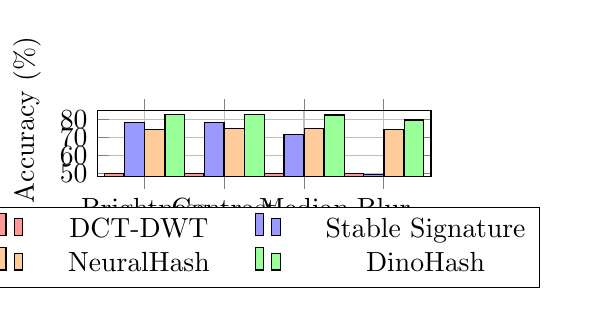
\begin{tikzpicture} 
\hspace{-0.5cm}
\begin{axis}[
    width=0.48\textwidth,
    height=0.2\textwidth,
    ylabel={Bit Accuracy (\%)},
    % xlabel={Transformation},
    xtick=data,
    symbolic x coords={Brightness, Contrast, Median, Blur},
    ybar=0.2,
    bar width=0.25cm,
    enlarge x limits={abs=0.6cm},
    legend style={
        at={(0.5,-0.45)},
        anchor=north,
        legend columns=2,
        column sep=0.5cm
    },
    ymin=48,
    ymax=85,
    grid=both
]
    % dct-dwt
    \addplot[fill=red!40] coordinates {
        (Brightness, 50)
        (Contrast, 50) 
        (Median, 50)
        (Blur, 50)
    };
    
    % Stable Signature
    \addplot[fill=blue!40] coordinates {
        (Brightness, 78.11)
        (Contrast, 78.14) 
        (Median, 71.7)
        (Blur, 49.38)
    };

    % NeuralHash
    \addplot[fill=orange!40] coordinates {
        (Brightness, 74.51)
        (Contrast, 74.79) 
        (Median, 74.96)
        (Blur, 74.35)
    };
    
    % DinoHash
    \addplot[fill=green!40] coordinates {
        (Brightness, 82.64)
        (Contrast, 82.69) 
        (Median, 82.45)
        (Blur, 79.63)
    };
    
    \legend{DCT-DWT, Stable Signature, NeuralHash, DinoHash}
\end{axis}
\end{tikzpicture}

\caption{\textbf{Bit Accuracy Comparison.} The mean bit accuracy of different methods after a simulated screenshot followed by the respective transformations.}
\label{fig:barplot}
\vspace{-0.5cm}
\end{figure}

\subsection{Distortion Robustness}

We use 1M randomly sampled images from the DiffusionDB dataset \cite{wang2023diffusiondblargescalepromptgallery} to carry out experiments for DCT-DWT watermarking, NeuralHash and our framework. We use 1M randomly sampled prompts of the dataset to generate images to benchmark Stable Signature.

\autoref{fig:roc} shows the Receiver Operating Characteristic (ROC) Curve for different hashing/watermarking methods under different transformations. The level of $\tau$ is varied from $0$ to $96$ to obtain different values for the TPR and FPR. The TPR is calculated by measuring the fraction of images whose degree of match, $M$, after the transformation equals or exceeds $\tau$. Conversely, the FPR is approximated using \autoref{eq:fpr} since it is too small to be measured experimentally. \autoref{fig:barplot} reports results on the mean bit accuracy of the algorithms. We do not include the TPR-FPR plot for DCT-DWT due to its near-random performance.

We observe that all algorithms are roughly equally robust to the brightness and contrast transformations due to their non-destructive nature. We also observe that DinoHash is significantly more robust to transformations than NeuralHash and Stable Signature across both metrics. We do not report the results for the vanilla (no transformation) case since any hashing method would trivially achieve a $100\%$ match in the cases without perturbations. This, however, does not always hold for watermarking methods since the watermark generation and extraction models may not always agree. Furthermore, all watermarking methods report the PSNR (Peak Signal-to-Noise Ratio) and SSIM (Structural Similarity Index) of the watermarked images. These metrics measure how perceptually similar the watermarked and the unwatermarked images are. Since hashing algorithms do not cause any modification to the underlying image, we achieve perfect PSNR and SSIM scores. Since NeuralHash is a proprietary algorithm, it is difficult to comment on why DinoHash performs better.
\begin{figure}[!h] 
    \centering
    \includegraphics[width=0.5\textwidth]{multi.png}
    \caption{\textbf{Detection Results.} The TPR/FPR detection curve of different methods after a simulated screenshot followed by the respective transformations, random erasing and text overlay.}
    \label{fig:roc}
    \vspace{-0.5cm}
\end{figure}


% \begin{table*}[t]
% \centering
% % \small
% \begin{adjustbox}{width=0.95\linewidth}  
% \setlength{\tabcolsep}{6pt} % Adjust column padding as needed
% \begin{tabular}{lccccccccc}
% \toprule
% {Method} & {Backbone} & {Resolution}&{Patch Size} & DALL-E 2 & DALL-E 3 & Firefly & Midjourney v5   & {AVG} \\ 

% \midrule
% \citet{cozzolino2024raising} & - & - &-& 0.706 / \textbf{0.612} & 0.794 / 0.639 & 0.766 / 0.635 & 0.698 / 0.602 & 0.741 / 0.622 \\
% \citet{corvi2023detection} & - & - & -& 0.689 / 0.502 & 0.287 / 0.500 & 0.574 / 0.501 & 0.481 / 0.500 & 0.508 / 0.501 \\
% \midrule
% \textit{Ours}-frozen \\
% \midrule
% DFN \cite{fang2023data} & ViT-H & 378 &14& 0.767 & \textbf{0.999} & \textbf{0.936} & \textbf{0.949} & \textbf{0.913} \\
% DFN \cite{fang2023data} & ViT-H & 224&14 & \textit{0.792} & 0.997 & 0.921 & 0.934 & \textit{0.911} \\
% SigLIP\cite{zhai2023sigmoid} & So-ViT-400M & 224&14 & 0.663 & 0.996 & 0.896 & 0.909 & 0.866 \\
% SigLIP\cite{zhai2023sigmoid} & So-ViT-400M & 384 &14& 0.731 & 0.997 & \textit{0.924} & 0.926 & 0.895 \\
% \midrule
% \textit{Ours}-finetuned \\
% \midrule
% DFN \cite{fang2023data} & ViT-H & 378&14 & 0.742 & 0.991 & 0.870 & 0.906 & 0.877 \\
% DFN \cite{fang2023data} & ViT-H & 224&14 & \textbf{0.818} & \textit{0.998} & 0.910 & 0.880 & 0.901 \\
% SigLIP\cite{zhai2023sigmoid} & So-ViT-400M & 224&14 & 0.781 & 0.997 & 0.887 & 0.937 & 0.901 \\
% SigLIP\cite{zhai2023sigmoid} & So-ViT-400M & 384&14 & 0.772 & 0.993 & 0.903 & \textit{0.938} & 0.902 \\
% \bottomrule
% \end{tabular}
% \end{adjustbox}
% \caption{AUC values for various methods across different models with average values.}
% \label{tab:auc_table}
% \end{table*}

\subsection{Experiments on DL detector}
\label{subsec:exp_dl}
\begin{table*}[t]
\centering
% \small
\begin{adjustbox}{width=0.95\linewidth}  
\setlength{\tabcolsep}{6pt} % Adjust column padding as needed
\begin{tabular}{lcccccccc}
\toprule
{Method} & {Backbone} & {Resolution} & DALL-E 2 & DALL-E 3 & Firefly & Midjourney v5   & {AVG} \\ 

\midrule
\citet{cozzolino2024raising} & - & - & 0.706 / \textbf{0.612} & 0.794 / 0.639 & 0.766 / 0.635 & 0.698 / 0.602 & 0.741 / 0.622 \\
\citet{corvi2023detection} & - & - &  0.689 / 0.502 & 0.287 / 0.500 & 0.574 / 0.501 & 0.481 / 0.500 & 0.508 / 0.501 \\
\midrule
\textit{Ours}-frozen \\
\midrule
DFN \cite{fang2023data} & ViT-H & 378 & 0.767 / 0.584 & \textbf{0.999} / \textbf{0.980} & \textbf{0.936} / \textbf{0.754} & \textbf{0.949} / \textbf{0.804} & \textbf{0.913} / \textbf{0.780} \\
DFN \cite{fang2023data} & ViT-H & 224& \textit{0.792} / \textit{0.605} & 0.997 / \textit{0.974} & 0.921 / 0.720 & 0.934 / 0.771 & \textit{0.911} / 0.767 \\
SigLIP\cite{zhai2023sigmoid} & So-ViT-400M & 224 & 0.663 / 0.574 & 0.996 / 0.965 & 0.896 / 0.730 & 0.909 / 0.785 & 0.866 / 0.764 \\
SigLIP\cite{zhai2023sigmoid} & So-ViT-400M & 384 & 0.731 / 0.600 & 0.997 / 0.972 & \textit{0.924} / \textit{0.742} & 0.926 / 0.772 & 0.895 / \textit{0.771} \\
\midrule
\textit{Ours}-finetuned \\
\midrule
DFN \cite{fang2023data} & ViT-H & 378 & 0.742 / 0.534 & 0.991 / 0.965 & 0.870 / 0.585 & 0.906 / 0.706 & 0.877 / 0.697 \\
DFN \cite{fang2023data} & ViT-H & 224 & \textbf{0.818} / 0.559 & \textit{0.998} / 0.972 & 0.910 / 0.623 & 0.880 / 0.689 & 0.901 / 0.711 \\
SigLIP\cite{zhai2023sigmoid} & So-ViT-400M & 224 & 0.781 / 0.542 & 0.997 / 0.966 & 0.887 / 0.620 & 0.937 / 0.737 & 0.901 / 0.716 \\
SigLIP\cite{zhai2023sigmoid} & So-ViT-400M & 384 & 0.772 / 0.592 & 0.993 / 0.966 & 0.903 / 0.664 & \textit{0.938} / 0.777 & 0.902 / 0.750 \\
\bottomrule
\end{tabular}
\end{adjustbox}
\caption{AUC/Accuracy scores for various methods across different commercial tools with average values. Accuracy values here are calculated with threshold of 0.5. \textbf{Bold} represent highest value in a column and \textit{italics} represent second highest value.}
\label{tab:auc_acc_table}
\end{table*}

% \begin{table*}[t]
% \centering
% % \small
% \begin{adjustbox}{width=0.95\linewidth} 
% \setlength{\tabcolsep}{5pt} % Adjust column padding as needed
% \begin{tabular}{lccccccccc}
% \toprule
% {Method} & {Backbone} & {Resolution} &{Patch Size} & DALL-E 2 & DALL-E 3 & Firefly & Midjourney v5 & {AVG} \\ 

% \midrule
% \citet{cozzolino2024raising} & - & - & -& \textbf{0.612} & 0.639 & 0.635 & 0.602 & 0.622 \\
% \citet{corvi2023detection} & - & - &-& 0.502 & 0.500 & 0.501 & 0.500 & 0.501 \\
% \midrule
% \textit{Ours}-frozen \\
% \midrule
% DFN \cite{fang2023data} & ViT-H & 378 &14& 0.584 & \textbf{0.980} & \textbf{0.754} & \textbf{0.804} & \textbf{0.780} \\
% DFN \cite{fang2023data} & ViT-H & 224 &14& \textit{0.605} & \textit{0.974} & 0.720 & 0.771 & 0.767 \\
% SigLIP\cite{zhai2023sigmoid} & So-ViT-400M & 224 &14& 0.574 & 0.965 & 0.730 & \textit{0.785} & 0.764 \\
% SigLIP\cite{zhai2023sigmoid} & So-ViT-400M & 384 &14& 0.600 & 0.972 & \textit{0.742} & 0.772 & \textit{0.771} \\
% \midrule
% \textit{Ours}-finetuned \\
% \midrule
% DFN \cite{fang2023data} & ViT-H & 378 &14& 0.534 & 0.965 & 0.585 & 0.706 & 0.697 \\
% DFN \cite{fang2023data} & ViT-H & 224 &14& 0.559 & 0.972 & 0.623 & 0.689 & 0.711 \\
% SigLIP\cite{zhai2023sigmoid} & So-ViT-400M & 224&14 & 0.542 & 0.966 & 0.620 & 0.737 & 0.716 \\
% SigLIP\cite{zhai2023sigmoid} & So-ViT-400M & 384 &14& 0.592 & 0.966 & 0.664 & 0.777 & 0.750 \\
% \bottomrule
% \end{tabular}
% \end{adjustbox}
% \caption{Accuracy values with 0.5 as threshold for various methods across different models with average values.}
% \label{tab:acc_table}
% \end{table*}

We fix a consistent setup to simulate real world conditions on a challenging dataset with postprocessing steps to evaluate our models as accurately as possible.

\noindent\textbf{Dataset} We report all results on the recently proposed Synthbuster dataset \cite{bammey2023synthbuster} as it has images from widely used commercial tools, i.e. Dalle2 \cite{dalle2}, Dalle3 \cite{dalle3}, Midjourneyv5 \cite{midjourney} and Adobe Firefly \cite{firefly}. It uses RAISE-1k \cite{dang2015raise} as its real part. Each source contains 1000 images. We use 10000 pairs of real and synthetic images for all training purposes. This set is created using the strategy proposed in \cite{cozzolino2024raising}. We randomly select 10000 images from the train set of COCO-2017\cite{lin2014microsoft}, generate their caption using BLIP \cite{li2022blip}, and generate images for these captions using Stable Diffusion XL \cite{podell2023sdxl}. We use a validation set of 500 pairs of images created similarly using the validation set of COCO-2017.
 
\noindent\textbf{Transformations} In real life, images often suffer cropping and compression when shared. We perform a set of transformations on all images to make the model more robust and to test its robustness under such attacks. We perform random crop to 62.5\% to 100\% of the original scale followed by resizing to 200x200 pixels. We then perform random jpeg compression to between 85\% to 100\% of initial quality.

\noindent\textbf{Testing Protocol} Our testing dataset contains synthetic images from four different sources having 1000 images each and a real set of 1000 images. While computing metrics for one synthetic image source, we consider just that subset of dataset and the real images. So, we effectively have 1000 synthetic and real images, making the dataset balanced.


\noindent\textbf{Metrics} We use area under ROC curve (AUC) and accuracy(ACC) with threshold of 0.5 as our metric. We use threshold of 0.5 to simulate a sitution where we have no prior information about the detector.

\noindent\textbf{Results} Our models outperform the previous SoTA~\cite{cozzolino2024raising} across both metrics. Linear SVM trained on top of frozen CLIP image encoder with ViT-H backbone, 378 input resolution and quickGELU activation function yields best results on most generators and on average. It shows improvements of 23.3\% / 25.4\% in AUC/ACC respectively over previous SoTA. Other models also perform better than~\citet{cozzolino2024raising}, we present detailed results in~\cref{tab:auc_acc_table}.
% and~\cref{tab:acc_table}.



% We also tried zero shot experiments leveraging the text encoder of CLIP for classification, but results were poor. More details in appendix. 

\begin{table}
\centering
\footnotesize
\setlength{\tabcolsep}{5pt} % Adjust column padding as needed
\begin{tabular}{lccccc}
\toprule
{Method} & {Backbone} & {Resolution} & {Epoch} & {LR} &{Batch Size} \\
\midrule
SigLIP \cite{zhai2023sigmoid} & So-ViT-400M & 384 & 5 & 5e-6& 8 \\ 
SigLIP \cite{zhai2023sigmoid} & So-ViT-400M & 224 & 3 & 5e-6&8 \\
DFN \cite{fang2023data} & ViT-H-14 & 378 & 4 & 5e-6&8 \\ 
DFN \cite{fang2023data} & ViT-H & 224 & 3 & 5e-6&8 \\ 
\bottomrule
\end{tabular}

\caption{Training configurations for various methods, including backbone, resolution, epochs, and learning rate.}
\label{tab:training_config}
\end{table}

\red{
\subsection{Searching pHash in the Database}
We have implemented our protocol as a PoC in an open-source library, available on GitHub. For this, we utilize Phantom Zone~\cite{PhantomZone}, an experimental library designed for the practical realization of MP-FHE. In our benchmarking scenario, the pHash values of the images stored in the database are encrypted using a shared key between two parties. This allows us to efficiently query and match encrypted pHash values, demonstrating the feasibility of our protocol in real-world applications.

In our implementation, we use the \texttt{FheBool} class from the PhantomZone library to perform homomorphic boolean logic. In this approach, each bit of the vectors is encrypted individually. As a result, encrypting a 96-bit vector involves creating 96 individual ciphertexts. A key advantage of treating each bit separately is the potential for parallelization during the evaluation phase of MP-FHE, which significantly speeds up the computation.

When a specific pHash value is queried, it is first encrypted locally by the client before being sent to the server for comparison with the encrypted database. The server then performs an XOR operation between the queried pHash value and each database entry. This operation is executed bit by bit and in parallel across all bits of the vectors. After the XOR operations are completed, the Hamming distance for each result is computed. This step is optimized using a 6-layer parallel boolean logic adder tree, which efficiently calculates the Hamming distance for all entries. If the distance for an entry is below the specified threshold (e.g., 8 bits), the result for that entry is set to True (1); otherwise, it is set to False (0). Once all entries are processed, the results are combined using a parallel OR tree. The final result is then sent back to the querying party for partial decryption. If the decrypted result is 1, it indicates that the queried pHash value is sufficiently similar to one or more entries in the encrypted database.


Table~\ref{tab:fhe_result} presents the average latency cost of determining whether two encrypted 96-bit vectors are close in FHEW, measured on a dataset with 1,000 entries. The table reports a cost breakdown of each phase of the FHEW evaluation. The columns ``XOR," ``HD," and ``Full Query" represent the average latency of calculating the XOR value, Hamming distance, and determining whether two 96-bit encrypted vectors are close or not, respectively. We conducted experiments on three different machines: 1) A midrange Dell Latitude 5531 with a 12$^{th}$ Gen Intel Core-i5 processor, 2) A Macbook Pro with a 10-core Apple Silicon M4 processor, and 3) A Google Cloud server equipped with 56 vCPUs and 112 GB memory running on an AMD EPYC 7B13 processor.

One of the key features of the proposed method is that each entry in the data is homomorphically encrypted using the same multi-party key. Consequently, FHE evaluations can be trustlessly distributed across multiple untrusted parties, as no single entity can leak or decrypt any data during query execution without access to all shared key fragments. This property enables the system to scale with minimal security considerations, making it cost-efficient. 

Although our current PoC implementation results indicate that a CPU-only device (without GPU acceleration) requires over 100 seconds to execute a query on a database with only 1,000 entries, the system can be scaled inexpensively by distributing computations across multiple trustless parties. The results from each party can then be merged using a parallel OR tree. The concept of clustering databases has also been utilized in previous work to enhance scalability~\cite{wally-search}.

\paragraph{\textbf{Related work.}} 
There are two categories of related work relevant to our constructions. The first group focuses on preserving the privacy of user queries against a database that is visible to the query executor~\cite{wally-search, tiptoe}. In such setups, it is crucial to ensure that the database owner cannot infer any information about the user's queries.

However, our system model is fundamentally different from these works. Specifically, in our target application, the database contains confidential user history that must remain undisclosed to any entity at all times. The key distinction is that, in our setting, even the data owner should not be able to reconstruct the query database. This constraint makes our protocol and the underlying problem significantly more complex than those addressed in~\cite{tiptoe, wally-search}.

Another line of work targets the same type of scenario as ours, where the database must remain unreconstructible due to its sensitive nature of stored data. The most notable recent work in this category are~\cite{iris-search, li2024panther}, in which the authors propose secretly sharing the original database among multiple parties, enabling user queries to be executed in an MPC-based manner. However, our MP-FHE-based protocol achieves stronger security guarantees. Notably:
\begin{compactitem}
    \item Query execution can be performed by any party, not just the shareholders.
    \item There are no costs associated with maintaining database shares, as the entire database remains encrypted and does not leak any information.
    \item No interaction is required among shareholders during query execution; the only interaction occurs when decrypting the final query result. This results in significantly lower communication complexity as pointed in recent work, such as~\cite{li2024panther}.
\end{compactitem}

\noindent
However, it is important to acknowledge that a pure MPC-based setup generally achieves higher performance compared to our FHE-based approach~\cite{li2024panther}. Therefore, while our construction represents an ideal and highly secure solution, it may not be practical for large-scale deployments. For this reason, we also extend and refine the protocol of~\cite{iris-search}, as discussed in Appendix~\ref{sec:apx-mpc}.

% In comparison with two TODO: double-check with phantom-zone. 

% in Tiptoe~\cite{?}, a private search engine, a single client query is 21 MB and requires 339 core-seconds of server computing against a database of 400 million entries. The high computational cost is because, for each client query, the server must scan the entire database; otherwise, it will learn which database entries the client is not interested in. Similarly, the client must send cryptographic material for each database entry, which results in high communication cost. An additional limitation of Tiptoe is that it requires each client to store a database-dependent state of around 50 MB for each client query. In wally protocol, the server computation and the communication are amortized over the number of clients making the requests; therefore, when the number of clients is large, the per-query cost becomes minimal. In Wally, the server learns a noised differentially private histogram of anonymized queries from all clients, over a partition of the server database. We emphasize that previous works, e.g., Tiptoe, are fully oblivious. That is, the server learns nothing besides that a particular client is making a query. Therefore, the privacy guarantee of schemes like Tiptoe is stronger than Wally. However, differential privacy is an accepted standard for strong privacy. 
}

\begin{table}[t]
\centering
\footnotesize
% \begin{threeparttable}
\red{
\begin{tabular}{cccccc}
\hline
System & CPU & Cores & XOR & HD & Full Query \\ \hline
Laptop & 12$^{th}$Gen i5 & 4 & 200 ms & 1.29 s & 1.3 s \\
Laptop & 12$^{th}$Gen i5 & 8 & 105 ms & 747 ms & 773 ms \\
Laptop & 12$^{th}$Gen i5 & 16 & 67 ms & 467 ms & 472 ms \\
MB Pro & Apple M4 & 10 & 59 ms & 421 ms &  440 ms \\
Server & AMD 7B13 & 56 & 26 ms & 134 ms & 137 ms \\ \hline
\end{tabular}
}
\caption{\red{The average latency cost of determining whether two encrypted 96-bit vectors are close in FHEW (Measured on a Dataset with 1,000 entries).}}
\label{tab:fhe_result}
\end{table}
